\title{Assignment 1: CS 663, Fall 2023}
\author{Darshan Makwana, Vignesh Nayak, Harsh Kavediya}
\date{Due: 25th August before 11:55 pm}

\documentclass[11pt]{article}
\usepackage{graphicx, caption}
\usepackage{amsmath}
\usepackage{amssymb}
\usepackage{hyperref}
\usepackage{ulem}
\usepackage[margin=0.5in]{geometry}
\begin{document}
\maketitle

\begin{enumerate}
\item[Q5.]
\begin{enumerate}

\item[(c)] \
\begin{figure}[!htb]
    \minipage{0.32\textwidth}
      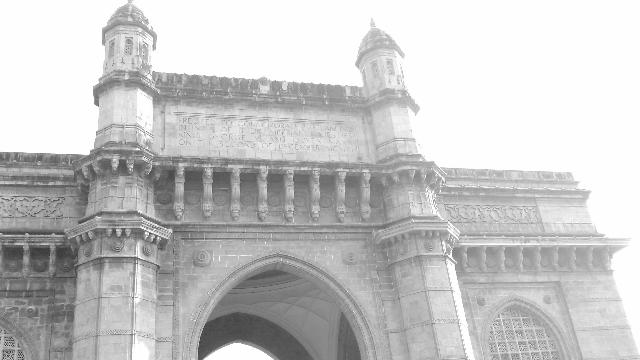
\includegraphics[width=\linewidth]{../assignment1/5/images/goi1.jpg}
      \caption*{goi1.jpg}
    \endminipage\hfill
    \minipage{0.32\textwidth}
      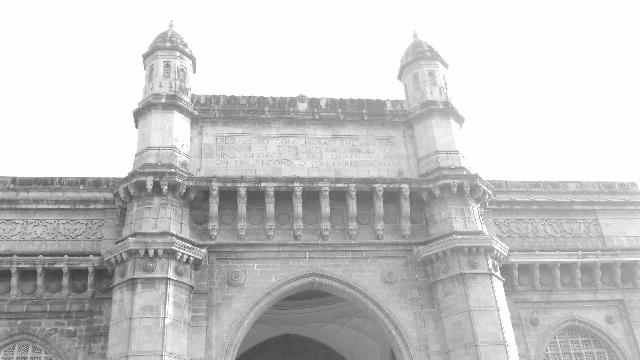
\includegraphics[width=\linewidth]{../assignment1/5/images/goi2.jpg}
      \caption*{goi2.jpg}
    \endminipage\hfill
    \minipage{0.32\textwidth}
      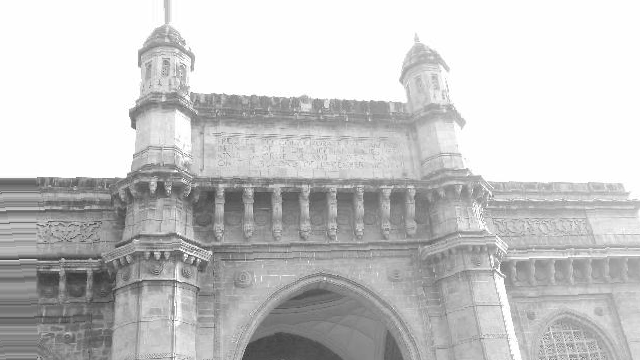
\includegraphics[width=\linewidth]{../assignment1/5/images/NNI.png}
      \caption*{Nearest Neighbour Interpolation of goi1.jpg}
    \endminipage
\end{figure}

\item[(d)] \
\begin{figure}[!htb]
    \minipage{0.32\textwidth}
      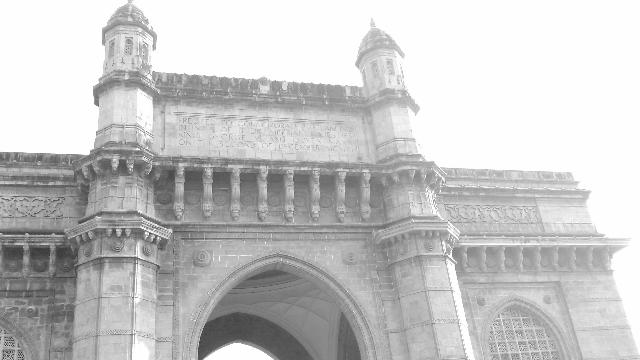
\includegraphics[width=\linewidth]{../assignment1/5/images/goi1.jpg}
      \caption*{goi1.jpg}
    \endminipage\hfill
    \minipage{0.32\textwidth}
      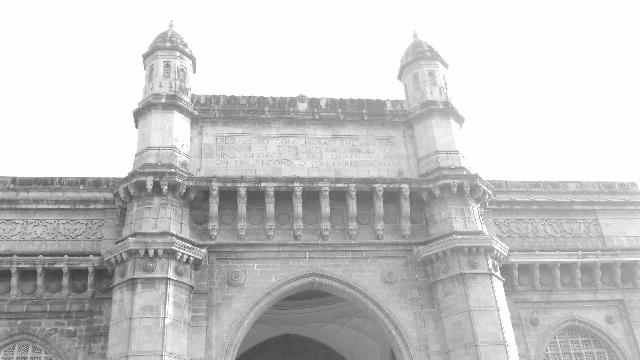
\includegraphics[width=\linewidth]{../assignment1/5/images/goi2.jpg}
      \caption*{goi2.jpg}
    \endminipage\hfill
    \minipage{0.32\textwidth}
      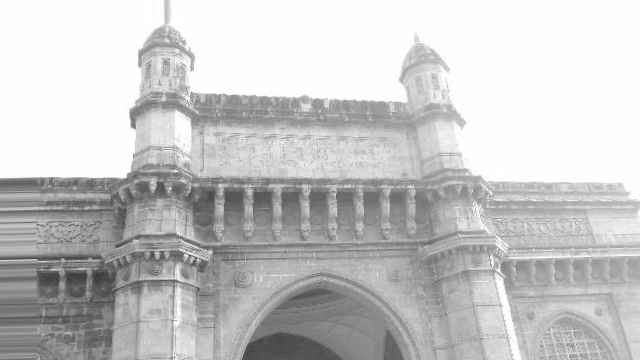
\includegraphics[width=\linewidth]{../assignment1/5/images/BI.png}
      \caption*{Bilinear Interpolation of goi1.jpg}
    \endminipage
\end{figure}

\item[(e)] If all the $n$ points selected are collinear (i.e they all lie on a straight line) then the system of linear equations
$$
\begin{bmatrix}
    x_{21} & x_{22} &.. & x_{2n} \\
    y_{21} & y_{22} &.. & y_{2n} \\
    1 & 1 &.. & 1
\end{bmatrix} = 
\begin{bmatrix}
    A_{11} & A_{12} & t_{x} \\
    A_{21} & A_{22} & t_{y} \\
    0 & 0 & 1
\end{bmatrix}
\begin{bmatrix}
    x_{11} & x_{12} &.. & x_{1n} \\
    y_{11} & y_{12} &.. & y_{1n} \\
    1 & 1 &.. & 1
\end{bmatrix}
$$
$$
X_{2} = AX_{1}
$$
becomes underactuated, as the rank of $X_{1}$ reduces to 2. While solving for A we multiply by $X_{1}^{T}$, which leaves us with $X_{2}X_{1}^{T}=AX_{1}X_{1}^{T}$. As $X_{1}X_{1}^{T}$ is non invertible there are infinitely many solutions of $A$. Thus the affine transformation matrix obtained can be any of those solutions.
In the revese warping procedure, inverse transformation matrix $A^{-1}$ maps the destination image to the line in the original image

\end{enumerate}
\end{enumerate}

\end{document}